\subsection{Caso d'uso UC9: Gestione dei questionari}
\label{UC9}
\begin{figure}[h]
	\centering
	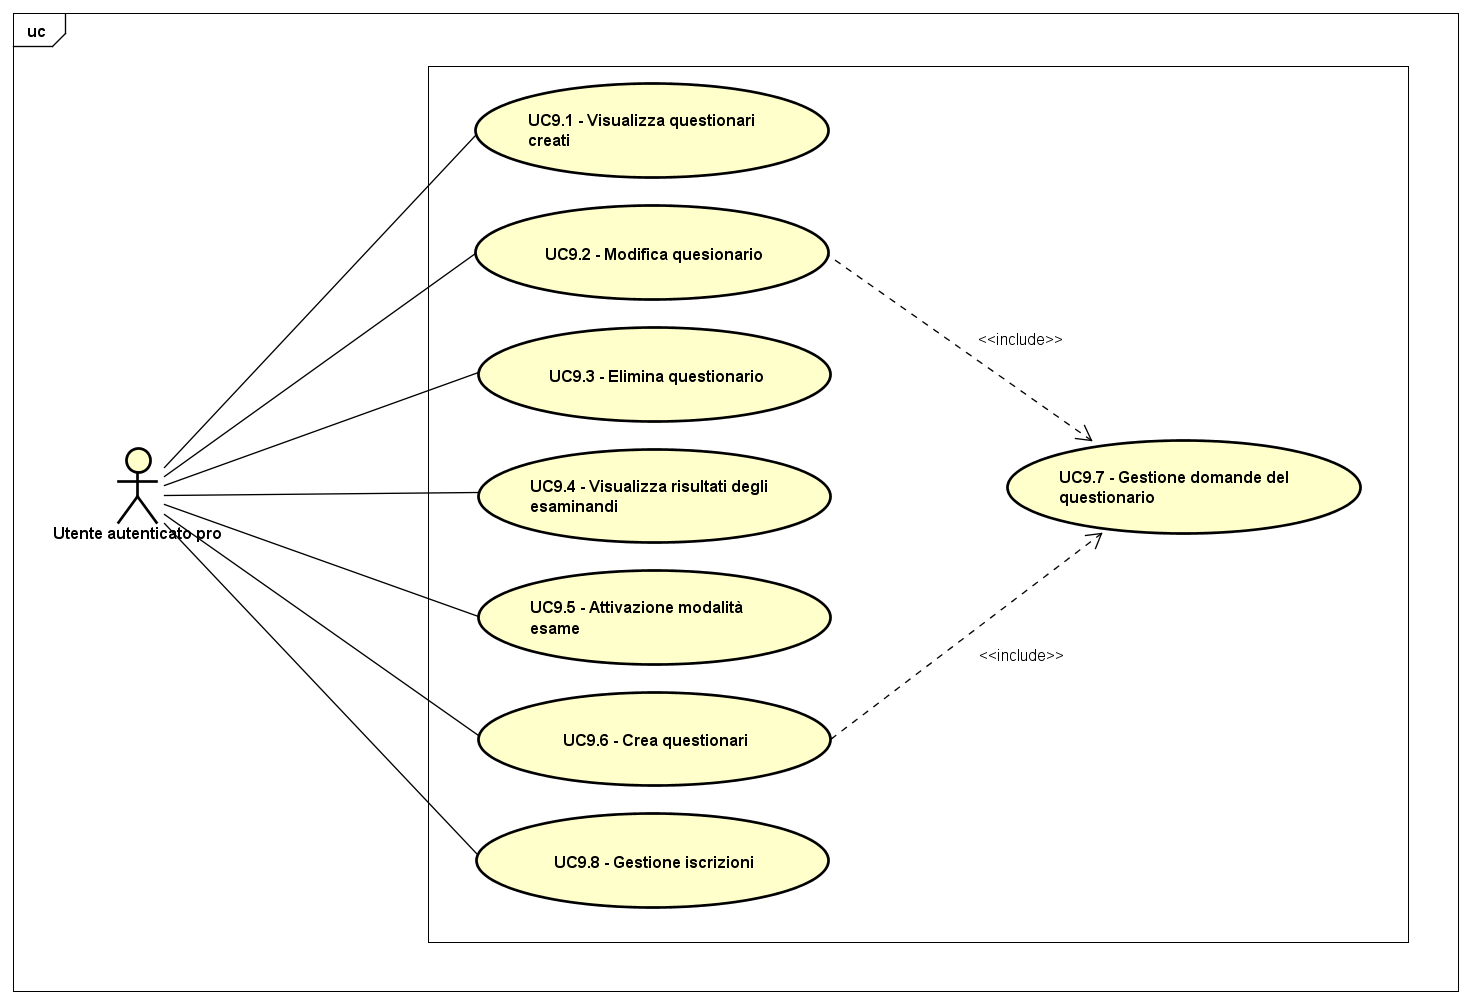
\includegraphics[scale=0.5,keepaspectratio]{UML/UC9.png}
	\caption{UC9: Gestione dei questionari}
\end{figure}
\FloatBarrier
\begin{itemize}
	\item \textbf{Attori}: \uaupro{};
	\item \textbf{Descrizione}: il sistema mostra una schermata in cui l'\uaupro{} può gestire i questionari. Può modificare e/o eliminare quelli creati da se stesso, crearne di nuovi, gestire le iscrizioni per i questionari ed infine attivare la modalità esame; 
	\item \textbf{Precondizione}: l'\uaupro{} accede al sito \textit{web\ped{G}} mediante ad un \textit{browser\ped{G}} supportato dal sistema. Seleziona tra le scelte possibili l'opzione "Gestione questionari" nelle opzioni del caso d'uso precedente;
	\item \textbf{Postcondizione}: il sistema ha eseguito le funzionalità scelte dall'\uaupro{};
	\item \textbf{Scenario principale}:
		\begin{enumerate}
			\item L'\uaupro{} può visualizzare i questionati creati (UC9.1);
			\item L'\uaupro{} può creare nuovi questionari (UC9.2);
			\item L'\uaupro{} può creare gestire le iscrizioni degli utenti per gli esami (UC9.4).
		\end{enumerate}
		\item \textbf{Inclusioni}: l'\uaupro{} può gestire le domande di un questionario (UC9.3).		
\end{itemize}
							
		\subsubsection{Caso d'uso UC9.1: Visualizza questionari creati}
		\label{UC9.1}
		\begin{figure}[h]
			\centering
		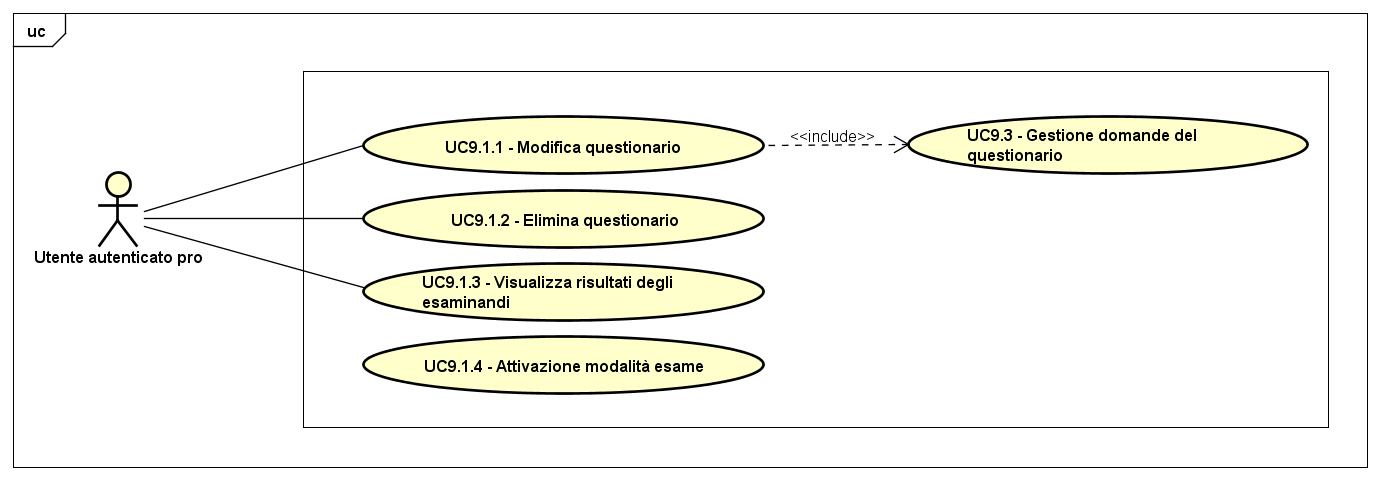
\includegraphics[scale=0.5,keepaspectratio]{UML/UC9_1.png}
			\caption{UC9.1: Visualizza questionari creati}
		\end{figure}
		\FloatBarrier
		\begin{itemize}
			\item \textbf{Attori}: \uaupro{};
			\item \textbf{Descrizione}: l'\uaupro{} può visualizzare i questionari da lui creati;
			\item \textbf{Precondizione}: l'\uaupro{} ha selezionato l'opzione "Visualizza questionari creati" tra le possibilità proposte in UC9;
			\item \textbf{Postcondizione}: il sistema ha eseguito le opzioni scelte dall'\uaupro{};
			\item \textbf{Scenario principale}: 
				\begin{enumerate}
					\item L'\uaupro{} può modificare un questionario creato (UC9.1.1);
					\item L'\uaupro{} può eliminare un questionario creato (UC9.1.2);
					\item L'\uaupro{} può visualizzare le statistiche degli esami compilati dagli esaminandi (UC9.1.3);
					\item L'\uaupro{} può attivare la modalità esame per un questionario (UC9.1.4).
				\end{enumerate}
				\item \textbf{Inclusioni}: l'\uaupro{} può gestire le domande di un questionario (UC9.3).
		\end{itemize}
		
			\subsubsection{Caso d'uso UC9.1.1: Modifica questionario}
			\label{UC9.1.1}
			\begin{figure}[h]
				\centering
			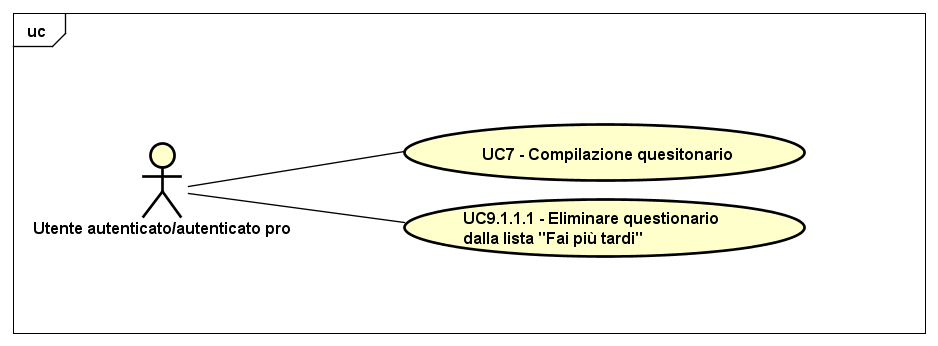
\includegraphics[scale=0.5,keepaspectratio]{UML/UC9_1_1.png}
				\caption{UC9.1.1: Modifica questionario}
			\end{figure}
			\FloatBarrier
			\begin{itemize}
				\item \textbf{Attori}: \uaupro{};
				\item \textbf{Descrizione}: l'\uaupro{} può modificare il questionario selezionato;
				\item \textbf{Precondizione}: l'\uaupro{} ha selezionato l'opzione "Modifica questionario" tra le possibilità proposte in UC9.1 su un questionario;
				\item \textbf{Postcondizione}: l'\uaupro{} ha modificato il questionario selezionato; 
				\item \textbf{Scenario principale}:
					\begin{enumerate}
						\item L'\uaupro{} può modificare il nome del questionario (UC9.1.1.1);
						\item L'\uaupro{} può confermare le modifiche apportare (UC9.1.1.2).
					\end{enumerate}
			\end{itemize}
								
					\subsubsection{Caso d'uso UC9.1.1.1: Modifica nome questionario}
					\label{UC9.1.1.1}
					\begin{itemize}
						\item \textbf{Attori}: \uaupro{};
						\item \textbf{Descrizione}: l'\uaupro{} può modificare il nome del questionario; 
						\item \textbf{Precondizione}: l'\uaupro{} ha selezionato l'opzione "Modifica nome questionario" tra le scelte possibili in UC9.1.1;
						\item \textbf{Postcondizione}: l'\uaupro{} ha modificato il nome del questionario; 
						\item \textbf{Scenario principale}: l'\uaupro{} modifica il nome del questionario.
					\end{itemize}
																					
					\subsubsection{Caso d'uso UC9.1.1.2: Conferma modifiche}
					\label{UC9.1.1.2}
					\begin{itemize}
						\item \textbf{Attori}: \uaupro{};
						\item \textbf{Descrizione}: l'\uaupro{} ha eseguito tutte le modifiche che voleva fare al questionario e ora deve salvarle in modo che siano archiviate;
						\item \textbf{Precondizione}: l'\uaupro{} ha selezionato l'opzione "Conferma modifiche" tra le scelte possibili in UC9.1.1;
						\item \textbf{Postcondizione}: l'\uaupro{} ha confermato le modifiche effettuate;
						\item \textbf{Scenario principale}: l'\uaupro{} conferma le modifiche effettuate;
						\item \textbf{Scenari alternativi}: l'\uaupro{} non conferma e le modifiche fatte non vengono salvate. L'\uaupro{} viene indirizzato alla pagina contenente la lista dei questionari da lui creati (UC9.1).
					\end{itemize}
										
			\subsubsection{Caso d'uso UC9.1.2: Elimina questionario}
			\label{UC9.1.2}
			\begin{figure}[h]
				\centering
			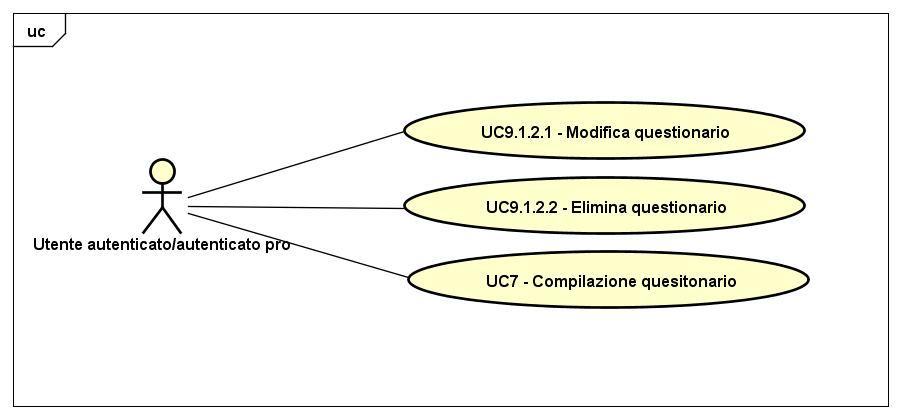
\includegraphics[scale=0.5,keepaspectratio]{UML/UC9_1_2.png}
				\caption{UC9.1.2: Elimina questionario}
			\end{figure}
			\FloatBarrier
			\begin{itemize}
				\item \textbf{Attori}: \uaupro{};
				\item \textbf{Descrizione}: l'\uaupro{} decide di voler eliminare il questionario dall'archivio dei questionari;
				\item \textbf{Precondizione}: l'\uaupro{} ha selezionato l'opzione "Elimina questionario" tra le scelte possibili in UC9.1;
				\item \textbf{Postcondizione}: l'\uaupro{} ha eliminato il questionario;
				\item \textbf{Scenario principale}: l'\uaupro{} deve confermare di voler eliminare il questionario (UC9.1.2.1).
			\end{itemize}
			
				\subsubsection{Caso d'uso UC9.1.2.1: Conferma eliminazione}
				\label{UC9.1.2.1}
				\begin{itemize}
					\item \textbf{Attori}: \uaupro{};
					\item \textbf{Descrizione}: l'\uaupro{} deve confermare di voler eliminare il questionario; 
					\item \textbf{Precondizione}: l'\uaupro{} ha selezionato l'opzione "Conferma eliminazione" tra le scelte possibili in UC9.1.2;
					\item \textbf{Postcondizione}: l'\uaupro{} ha confermato di voler eliminare il questionario;
					\item \textbf{Scenario principale}: l'\uaupro{} conferma di voler eliminare il questionario;
					\item \textbf{Scenari alternativi}: l'\uaupro{} non conferma di voler eliminare il questionario. L'\uaupro{} viene indirizzato alla pagina contenente la lista dei questionari da lui creati (UC9.1).
				\end{itemize}
								
		\subsubsection{Caso d'uso UC9.1.3: Visualizza risultati degli esaminandi}
		\label{UC9.1.3}
		\begin{itemize}
			\item \textbf{Attori}: \uaupro{};
			\item \textbf{Descrizione}: l'\uaupro{} può visualizzare le statistiche relative all'esito di un  questionario compilato dagli esaminandi;
			\item \textbf{Precondizione}: l'\uaupro{} ha selezionato l'opzione "Visualizza risultati degli esaminandi" tra le possibilità proposte in UC9.1;
			\item \textbf{Postcondizione}: il sistema ha eseguito le opzioni scelte dall'\uaupro{};
			\item \textbf{Scenario principale}: l'\uaupro{} visualizza le statistiche relative all'esito di un questionario compilato dagli esaminandi. 
		\end{itemize}
		
		\subsubsection{Caso d'uso UC9.1.4: Attivazione modalità esame}
		\label{UC9.1.4}
		\begin{itemize}
			\item \textbf{Attori}: \uaupro{};
			\item \textbf{Descrizione}: l'\uaupro{} può attivare l'esame cosicché esso sia compilabile dagli \uau{} iscritti;
			\item \textbf{Precondizione}: l'\uaupro{} ha selezionato l'opzione " Attivazione modalità esame" tra le possibilità proposte in UC9.1 su un questionario;
			\item \textbf{Postcondizione}: il sistema ha attivato l'esame cosicché esso possa essere compilato dagli \uaus{} iscritti;
			\item \textbf{Scenario principale}: l'\uaupro{} attiva l'esame cosicché esso possa essere compilato dagli \uaus{} iscritti.
		\end{itemize}
										
	\subsubsection{Caso d'uso UC9.2: Crea questionari}
	\label{UC9.2}
	\begin{figure}[h]
		\centering
	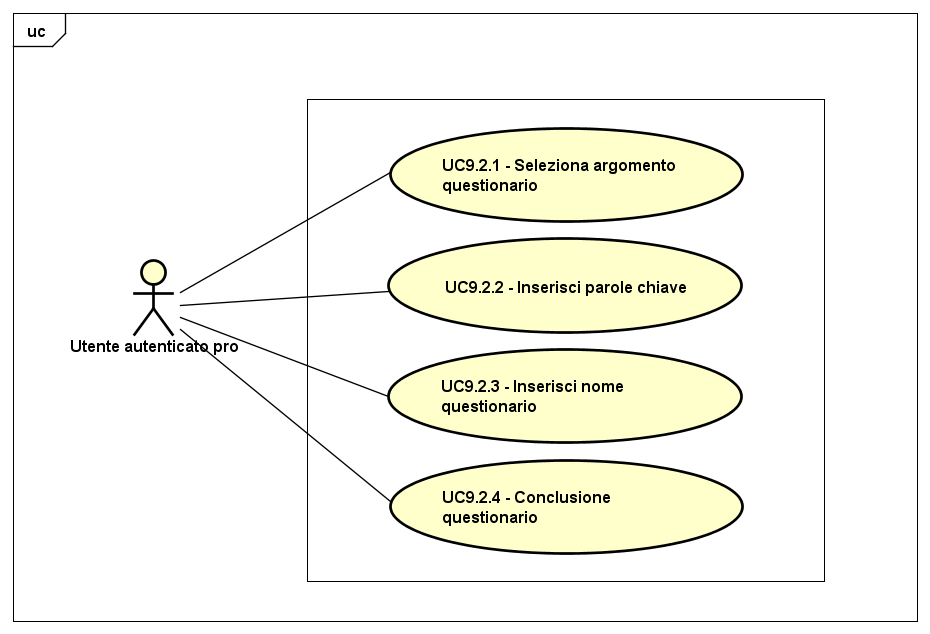
\includegraphics[scale=0.5,keepaspectratio]{UML/UC9_2.png}
		\caption{UC9.2: Crea questionari}
	\end{figure}
	\FloatBarrier
	\begin{itemize}
		\item \textbf{Attori}: \uaupro{};
		\item \textbf{Descrizione}: l'\uaupro{} può creare un nuovo questionario; 
		\item \textbf{Precondizione}: l'\uaupro{} ha selezionato l'opzione "Crea questionari" tra le possibilità proposte in UC9;
		\item \textbf{Postcondizione}: l'\uaupro{} ha creato un questionario;
		\item \textbf{Scenario principale}:
			\begin{enumerate}
				\item L'\uaupro{} può selezionare l'argomento del questionario (UC9.2.1);
				\item L'\uaupro{} può inserire il nome del questionario (UC9.2.2);
				\item L'\uaupro{} può selezionare gli argomenti del questionario (UC9.2.3);
				\item L'\uaupro{} può concludere il questionario (UC9.2.4).
			\end{enumerate}
		\end{itemize}
	
		\subsubsection{Caso d'uso UC9.2.1: Seleziona argomento questionario}
		\label{UC9.2.1}
		\begin{itemize}
			\item \textbf{Attori}: \uaupro{};
			\item \textbf{Descrizione}: l'\uaupro{} può selezionare l'argomento del questionario; 
			\item \textbf{Precondizione}: l'\uaupro{} ha selezionato l'opzione "Seleziona tipologia questionario" tra le scelte possibili in UC9.2;
			\item \textbf{Postcondizione}: l'\uaupro{} ha selezionato l'argomento del questionario;
			\item \textbf{Scenario principale}: l'\uaupro{} seleziona l'argomento del questionario.
		\end{itemize}
		
		\subsubsection{Caso d'uso UC9.2.2: Inserisci parole chiave}
		\label{UC9.2.2}
		\begin{itemize}
			\item \textbf{Attori}: \uaupro{};
			\item \textbf{Descrizione}: l'\uaupro{} può inserire delle parole chiave che identifichino il questionario; 
			\item \textbf{Precondizione}: l'\uaupro{} ha selezionato l'opzione "Inserisci parole chiave" tra le scelte possibili in UC9.2;
			\item \textbf{Postcondizione}: l'\uaupro{} ha inserito delle parole chiave fino ad un massimo di quattro; 
			\item \textbf{Scenario principale}: l'\uaupro{} inserisce le parole chiave che identificano il questionario.
		\end{itemize}
			
		\subsubsection{Caso d'uso UC9.2.3: Inserisci nome questionario}
		\label{UC9.2.3}
		\begin{itemize}
			\item \textbf{Attori}: \uaupro{};
			\item \textbf{Descrizione}: l'\uaupro{} può inserire il nome del questionario; 
			\item \textbf{Precondizione}: l'\uaupro{} ha selezionato l'opzione "Inserisci nome questionario" tra le scelte possibili in UC9.2;
			\item \textbf{Postcondizione}: l'\uaupro{} ha inserito il nome del questionario; 
			\item \textbf{Scenario principale}: l'\uaupro{} inserisce il nome del questionario.
		\end{itemize}
				
		\subsubsection{Caso d'uso UC9.2.4: Conclusione questionario}
		\label{UC9.2.4}
		\begin{figure}[h]
			\centering
			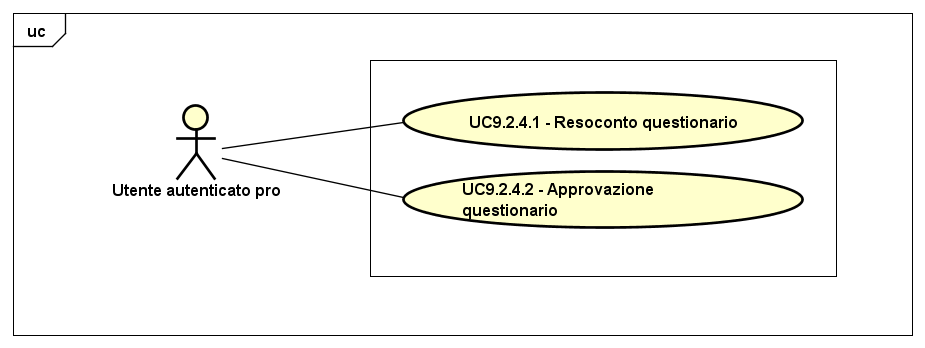
\includegraphics[scale=0.5,keepaspectratio]{UML/UC9_2_4.png}
			\caption{UC9.2.4: Conclusione questionario}
		\end{figure}
		\FloatBarrier
		\begin{itemize}
			\item \textbf{Attori}: \uaupro{}; 
			\item \textbf{Descrizione}: l'\uaupro{} decide che il questionario è concluso;
			\item \textbf{Precondizione}: l'\uaupro{} ha scelto l'opzione "Conclusione questionario" tra le scelte possibili in UC9.2;
			\item \textbf{Postcondizione}: l'\uaupro{} ha completato il questionario;
			\item \textbf{Scenario principale}: 
				\begin{enumerate}
					\item L'\uaupro{} visualizza il riepilogo finale del questionario appena creato (UC9.2.4.1); 
					\item L'\uaupro{} approva la creazione del questionario (UC9.2.4.2).
				\end{enumerate}
		\end{itemize}
				
			\subsubsection{Caso d'uso UC9.2.4.1: Resoconto questionario}
			\label{UC9.2.4.1}
			\begin{itemize}
				\item \textbf{Attori}: \uaupro{};
				\item \textbf{Descrizione}: l'\uaupro{} visualizza le scelte fatte finora durante la creazione del questionario;
				\item \textbf{Precondizione}: l'\uaupro{} ha scelto l'opzione "Resoconto questionario" tra le scelte possibili in UC9.2.4;
				\item \textbf{Postcondizione}: l'\uaupro{} ha visualizzato le scelte fatte finora durante la creazione del questionario;
				\item \textbf{Scenario principale}: l'\uaupro{} visualizza le scelte fatte finora durante la creazione del questionario.
			\end{itemize}
			
			\subsubsection{Caso d'uso UC9.2.4.2: Approvazione questionario}
			\label{UC9.2.4.2}
			\begin{itemize}
				\item \textbf{Attori}: \uaupro{};
				\item \textbf{Descrizione}: l'\uaupro{} deve approvare il questionario appena creato;
				\item \textbf{Precondizione}: l'\uaupro{} ha scelto l'opzione "Approvazione questionario" tra le scelte possibili in UC9.2.4; 
				\item \textbf{Postcondizione}: l'\uaupro{} ha approvato il questionario;
				\item \textbf{Scenario principale}: l'\uaupro{} approva il questionario;
				\item \textbf{Scenari alternativi}: l'\uaupro{} non approva il questionario e quest'ultimo non viene archiviato. L'\uaupro{} viene mandato alla pagina precedente.
			\end{itemize}				
	 
	 \subsubsection{Caso d'uso UC9.3: Gestione domande del questionario}
	 \label{UC9.3}
	 \begin{figure}[h]
	 	\centering
	 	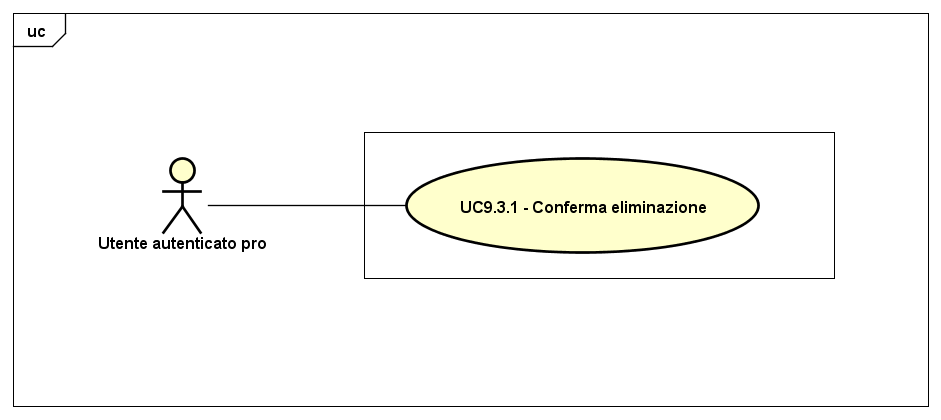
\includegraphics[scale=0.5,keepaspectratio]{UML/UC9_3.png}
	 	\caption{UC9.3: Gestione domande del questionario}
	 \end{figure}
	 \FloatBarrier
	 \begin{itemize}
	 	\item \textbf{Attori}: \uaupro{};
	 	\item \textbf{Descrizione}: l'\uaupro{} può gestire le domande di un proprio questionario, aggiungendone oppure togliendone;
	 	\item \textbf{Precondizione}: l'\uaupro{} ha selezionato l'opzione "Gestione domande" tra le scelte possibili in UC9.1.1 oppure in UC9.2;
	 	\item \textbf{Postcondizione}: l'\uaupro{} ha gestito le domande di un questionario;
	 	\item \textbf{Scenario principale}: 
	 	\begin{enumerate}
	 		\item L'\uaupro{} aggiunge altre domande (UC9.3.1);
	 		\item L'\uaupro{} elimina una domanda (UC9.3.2).
	 	\end{enumerate}
	 	\item \textbf{Inclusioni}: l'\uaupro{} può creare delle nuove domande per il questionario (UC8.1).		
	 \end{itemize}
	 
		 \subsubsection{Caso d'uso UC9.3.1: Aggiungi altre domande}
		 \label{UC9.3.1}
		 \begin{figure}[h]
		 	\centering
		 	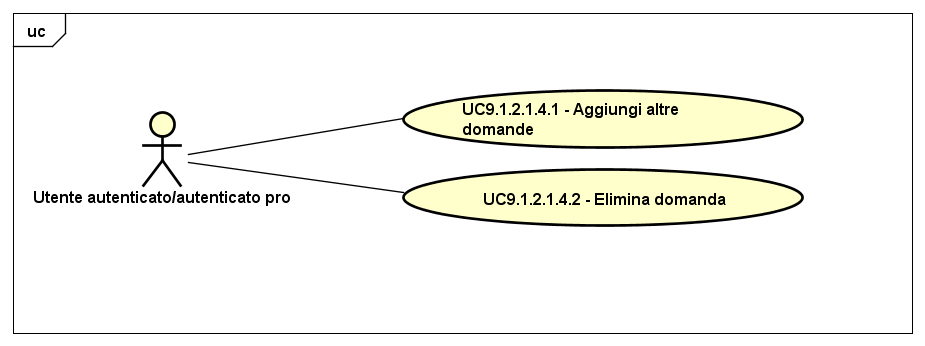
\includegraphics[scale=0.5,keepaspectratio]{UML/UC9_3_1.png}
		 	\caption{UC9.3.1: Aggiungi altre domande}
		 \end{figure}
		 \FloatBarrier
		 \begin{itemize}
		 	\item \textbf{Attori}: \uaupro{};
		 	\item \textbf{Descrizione}: l'\uaupro{} può aggiungere altre domande cercando tra quelle già memorizzate nell'archivio oppure creandone una nuova; 
		 	\item \textbf{Precondizione}: l'\uaupro{} ha selezionato l'opzione "Aggiungi altre domande" tra le scelte possibili in UC9.3;
		 	\item \textbf{Postcondizione}: l'\uaupro{} ha aggiunto nuove domande;
		 	\item \textbf{Scenario principale}: l'\uaupro{} può eseguire una ricerca nelle domande archiviate (UC9.3.1.1).
		 \end{itemize}
		 
		 \subsubsection{Caso d'uso UC9.3.1.1: Ricerca domande}
		 \label{UC9.3.1.1}
		 \begin{figure}[h]
		 	\centering
		 	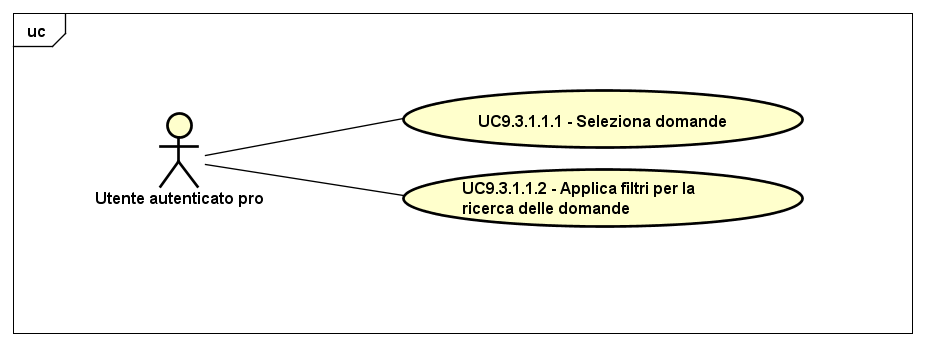
\includegraphics[scale=0.5,keepaspectratio]{UML/UC9_3_1_1.png}
		 	\caption{UC9.3.1.1: Ricerca domande}
		 \end{figure}
		 \FloatBarrier
		 \begin{itemize}
		 	\item \textbf{Attori}: \uaupro{};
		 	\item \textbf{Descrizione}: l'\uaupro{} può eseguire una ricerca tra le domande archiviate; 
		 	\item \textbf{Precondizione}: l'\uaupro{} ha selezionato l'opzione "Ricerca domande" tra le scelte possibili in UC9.3.1;
		 	\item \textbf{Postcondizione}: l'\uaupro{} ha ricercato tra le domande archiviate;
		 	\item \textbf{Scenario principale}:
		 	\begin{enumerate}
		 		\item L'\uaupro{} può selezionare le domande (UC9.3.1.1.1); 
		 		\item L'\uaupro{} può applicare dei filtri per la ricerca delle domande (UC9.3.1.1.2).
		 	\end{enumerate}
		 	\item \textbf{Scenari alternativi}: nel caso in cui non ci sia nessun risultato dalla ricerca all'\uaupro{} viene proposta la possibilità di creare una nuova domanda (UC8.1).
		 \end{itemize}
		 
		 \subsubsection{Caso d'uso UC9.3.1.1.1: Seleziona domande}
		 \label{UC9.3.1.1.1}
		 \begin{itemize}
		 	\item \textbf{Attori}: \uaupro{};
		 	\item \textbf{Descrizione}: l'\uaupro{} può selezionare le domande tra quelle ottenute dalla ricerca;
		 	\item \textbf{Precondizione}: l'\uaupro{} ha ottenuto una lista di risultati;
		 	\item \textbf{Postcondizione}: l'\uaupro{} ha selezionato delle domande; 
		 	\item \textbf{Scenario principale}: l'\uaupro{} seleziona le domande.
		 \end{itemize}
		 
		 \subsubsection{Caso d'uso UC9.3.1.1.2: Applica filtri per la ricerca delle domande}
		 \label{UC9.3.1.1.2}
		 \begin{itemize}
		 	\item \textbf{Attori}: \uaupro{};
		 	\item \textbf{Descrizione}: l'\uaupro{} può applicare dei filtri per ottenere dei risultati migliori nelle ricerche. 
			 	\begin{itemize}
					\item Selezionare la difficoltà delle domande;
					\item Ordinarle per difficoltà;
					\item Ordinarle per parola chiave;
					\item Visualizzare quelle create da se stessi.
			 	\end{itemize}
		 	\item \textbf{Precondizione}: l'\uaupro{} ha selezionato l'opzione "Applica filtri per la ricerca delle domande" tra le scelte possibili in UC9.3.1.1;
		 	\item \textbf{Postcondizione}: l'\uaupro{} ha applicato dei filtri per la ricerca; 
		 	\item \textbf{Scenario principale}: l'\uaupro{} seleziona dei filtri da applicare per la ricerca.
		 \end{itemize}
		 
		 \subsubsection{Caso d'uso UC9.3.2: Elimina domanda dal questionario}
		 \label{UC9.3.2}
		 \begin{figure}[h]
		 	\centering
		 	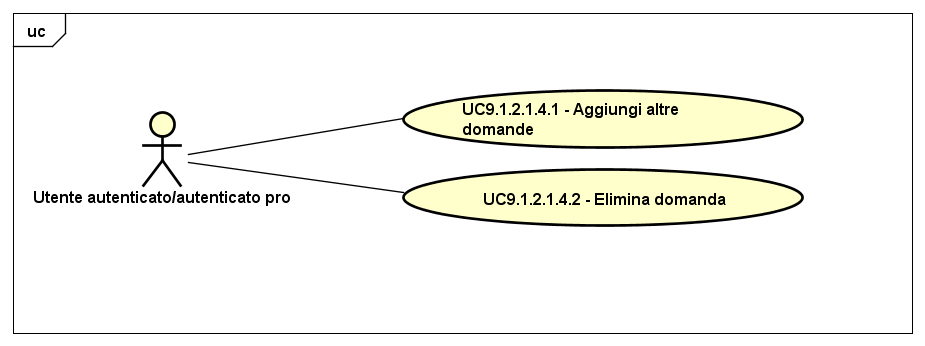
\includegraphics[scale=0.5,keepaspectratio]{UML/UC9_3_2.png}
		 	\caption{UC9.3.2: Elimina domanda dal questionario}
		 \end{figure}
		 \FloatBarrier
		 \begin{itemize}
		 	\item \textbf{Attori}: \uaupro{};
		 	\item \textbf{Descrizione}: l'\uaupro{} può eliminare una domanda da un questionario;
		 	\item \textbf{Precondizione}: l'\uaupro{} ha selezionato l'opzione "Elimina domanda" tra le scelte possibili in UC9.3;
		 	\item \textbf{Postcondizione}: l'\uaupro{} ha eliminato una domanda;
		 	\item \textbf{Scenario principale}: l'\uaupro{} deve confermare di voler eliminare la domanda (UC9.3.2.1); 
		 	\item \textbf{Scenari alternativi}: l'\uaupro{} ha cancellato tutte le domande. Deve allora inserirne almeno una, viene allora rimandato a UC9.3.1.
		 \end{itemize}
		 
		 \subsubsection{Caso d'uso UC9.3.2.1: Conferma eliminazione domanda}
		 \label{UC9.3.2.1}
		 \begin{itemize}
		 	\item \textbf{Attori}: \uaupro{};
		 	\item \textbf{Descrizione}: l'\uaupro{} deve confermare di voler eliminare la domanda;
		 	\item \textbf{Precondizione}: l'\uaupro{} ha deciso di voler eliminare la domanda;
		 	\item \textbf{Postcondizione}: l'\uaupro{} ha eliminato una domanda;
		 	\item \textbf{Scenario principale}: l'\uaupro{} conferma di voler eliminare la domanda;
		 	\item \textbf{Scenari alternativi}: l'\uaupro{} annulla l'eliminazione della domanda, viene allora rimandato a UC9.3.
		 \end{itemize}
		 
	 \subsubsection{Caso d'uso UC9.4: Gestione iscrizioni}
	 \label{UC9.4}
	 \begin{figure}[h]
	 	\centering
	 	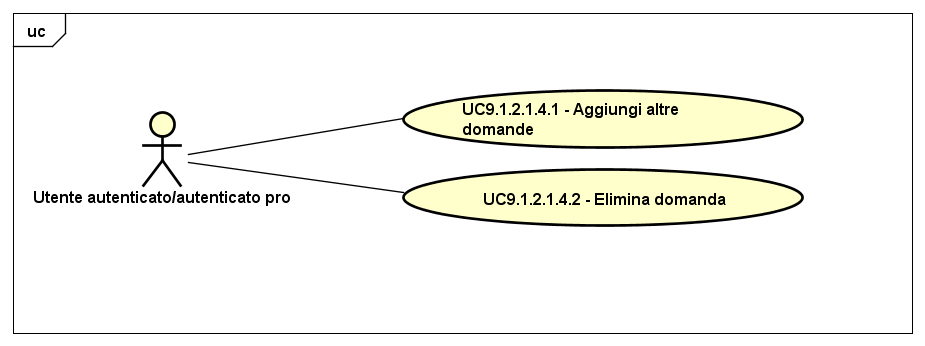
\includegraphics[scale=0.5,keepaspectratio]{UML/UC9_4.png}
	 	\caption{UC9.4: Gestione iscrizioni}
	 \end{figure}
	 \FloatBarrier
	 \begin{itemize}
	 	\item \textbf{Attori}: \uaupro{};
	 	\item \textbf{Descrizione}: l'\uaupro{} per far in modo che gli utenti partecipino ad un suo questionario deve approvare la loro iscrizione;
	 	\item \textbf{Precondizione}: l'\uaupro{} ha selezionato l'opzione "Gestione iscrizioni" tra le scelte possibili in UC9.3;
	 	\item \textbf{Postcondizione}: l'\uaupro{} ha approvato la partecipazione degli utenti che vogliono prendere parte al questionario;
	 	\item \textbf{Scenario principale}: l'\uaupro{} seleziona quale questionario gestire (UC9.4.1).
	 \end{itemize}
	 
		 \subsubsection{Caso d'uso UC9.4.1: Seleziona questionario}
		 \label{UC9.4.1}
		 \begin{figure}[h]
		 	\centering
		 	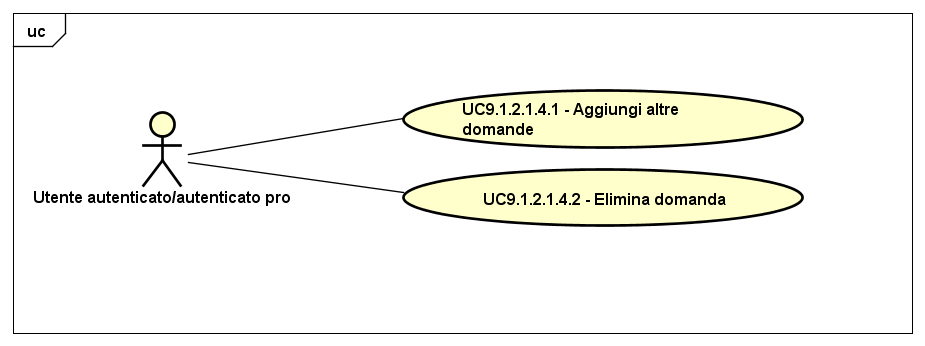
\includegraphics[scale=0.5,keepaspectratio]{UML/UC9_4_1.png}
		 	\caption{UC9.4.1: Seleziona questionario}
		 \end{figure}
		 \FloatBarrier
		 \begin{itemize}
		 	\item \textbf{Attori}: \uaupro{};
		 	\item \textbf{Descrizione}: l'\uaupro{} ha selezionato il questionario del quale vuole approvare l'iscrizione degli utenti che voglio prenderne parte. Di questo ne visualizzerà l'elenco degli utenti che hanno richiesto la partecipazione; 
		 	\item \textbf{Precondizione}: l'\uaupro{} ha selezionato l'opzione "Seleziona questionario" tra le scelte possibili in UC9.3;
		 	\item \textbf{Postcondizione}: l'\uaupro{} ha selezionato quale questionario gestire;
		 	\item \textbf{Scenario principale}: l'\uaupro{} deve decidere quali utenti, tra quelli che vogliono partecipare, iscrivere al questionario (UC9.4.1.1).
		 \end{itemize}
		 
			 \subsubsection{Caso d'uso UC9.4.1.1: Accettazione iscrizione utente}
			 \label{UC9.4.1.1}
			 \begin{itemize}
			 	\item \textbf{Attori}: \uaupro{};
			 	\item \textbf{Descrizione}: l'\uaupro{} decide quali utenti, tra quelli che vogliono partecipare al questionario, accettare; 
			 	\item \textbf{Precondizione}: l'\uaupro{} ha selezionato l'opzione "Accettazione iscrizione utente" tra le scelte possibili in UC9.4.1 su un particolare \uaupro{} che vuole partecipare ad un questionario;
			 	\item \textbf{Postcondizione}: l'\uaupro{} ha approvato la partecipazione degli utenti che chiedono di iscriversi al questionario;
			 	\item \textbf{Scenario principale}: l'\uaupro{} approva l'\uau{} o l'\uaupro{} che ha fatto richiesta per la partecipazione al questionario; 
			 	\item \textbf{Scenari alternativi}: nel caso in cui un \uau{} o \uaupro{} che vuole partecipare, non venga approvato, esso non avrà possibilità di accedere al questionario e ne sarà escluso.
			 \end{itemize}
			
				